%!TEX root = ../thesis.tex
%*******************************************************************************
%                                   Context                                    %
%*******************************************************************************

\chapter{Project Context}

\ifpdf
    \graphicspath{{2.0-Context/Figs/Raster/}{2.0-Context/Figs/PDF/}{2.0-Context/Figs/}}
\else
    \graphicspath{{2.0-Context/Figs/Vector/}{2.0-Context/Figs/}}
\fi

\section{Context}
- pfe \\
- Engineering degree

\section{Host company}
- iExec: founded when where, size, doing what \dots

\section{Problematic}
- Enegy Consumption \\
- Centralized Services \\
- Idle IoT devices \\
- Idle Computing resources 

\section{Suggested Solution}
- Positive Energy Worker
- Usefull use cases
- Multi-functionality IoT devices

\section{Adopted Methodology}
- To Do

\clearpage

\tochide\section{Hidden section}
\textbf{Lorem ipsum dolor sit amet}, \textit{consectetur adipiscing elit}. In mag a dignissim nisl iaculis nec. Praes et tempus mi cursus.

Etiam elementum eleifend sed \footnote{My footnote goes blah blah blah! \dots}. Maecenas dapibu augue ut urna Integer non dictum nunc.


\begin{landscape}

\section*{Subplots}
I can cite Wall-E (see Fig.~\ref{fig:WallE}) and Minions in despicable me (Fig.~\ref{fig:Minnion}) or I can cite the whole figure as Fig.~\ref{fig:animations}

\begin{figure}
  \centering
  \begin{subfigure}[b]{0.3\textwidth}
    
\includegraphics[width=\textwidth]{TomandJerry}
    \caption{Tom and Jerry}
    \label{fig:TomJerry}   
  \end{subfigure}             
  \begin{subfigure}[b]{0.3\textwidth}
    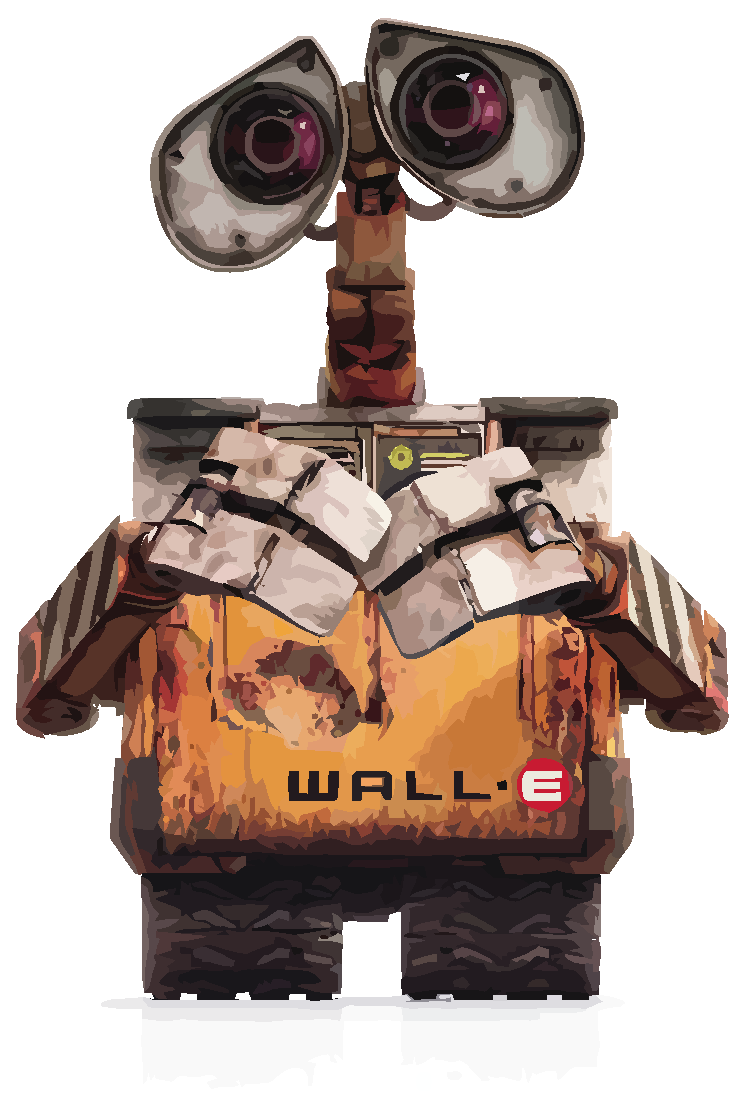
\includegraphics[width=\textwidth]{WallE}
    \caption{Wall-E}
    \label{fig:WallE}
  \end{subfigure}             
  \begin{subfigure}[b]{0.3\textwidth}
    
\includegraphics[width=\textwidth]{minion}
    \caption{Minions}
    \label{fig:Minnion}
  \end{subfigure}
  \caption{Best Animations}
  \label{fig:animations}
\end{figure}


\end{landscape}
